\documentclass{article}

\PassOptionsToPackage{numbers, compress}{natbib}

\usepackage[preprint]{neurips_2025}

\usepackage[utf8]{inputenc}
\usepackage[T1]{fontenc}
\usepackage{hyperref}
\usepackage{url}
\usepackage{booktabs}
\usepackage{amsmath}
\usepackage{amsfonts}
\usepackage{amssymb}
\usepackage{nicefrac}
\usepackage{microtype}
\usepackage{xcolor}
\usepackage{graphicx}
\usepackage{array}
\usepackage{caption}
\usepackage{multirow}

\captionsetup{font=small,labelfont=bf,skip=2pt}

\definecolor{accent}{HTML}{0072B2}
\definecolor{warn}{HTML}{D55E00}
\definecolor{good}{HTML}{009E73}
\hypersetup{colorlinks=true,urlcolor=accent,linkcolor=accent,citecolor=accent}

\newcommand{\keyfact}[1]{\textcolor{accent}{\textbf{#1}}}
\newcommand{\lever}[1]{\textcolor{warn}{\textbf{#1}}}

\title{Revenue System Diagnosis: A Prescriptive EDA for an 18-Month Forecast of a Vietnamese Fashion E-Commerce Company}

\author{%
  The Gridbreakers \\
  Datathon 2026 --- Part 2 \\
  \texttt{team@gridbreakers.vn} \\
}


\begin{document}


\maketitle


\begin{abstract}
We diagnose 10.5 years (3{,}833 daily observations, 14 relational tables) of a Vietnamese fashion e-commerce business under a single clinical question: \emph{what do we need to know to forecast the next 548 days?} Three findings overturn conventional intuition. (i)~A \textbf{40.5\% regime drop occurred in 2019, before COVID} (Welch $t{=}28.6$, $p{<}10^{-160}$, Cohen's $d{=}0.89$); (ii)~the peak is \textbf{May, $+53\%$ above the grand mean} --- not Q4, which is the trough at $-41\%$; (iii)~\textbf{heavy-promo days have 13.3\% lower median revenue} (Mann-Whitney $U$, $p{=}1.4\times10^{-12}$), evidence of defensive rather than offensive couponing. Two structural risks compound: 80.1\% of revenue sits in a single category (HHI $=0.67$), and stockout and overstock coexist at 60--87\% of SKUs --- an allocation, not a supply problem. We translate each diagnosis into a quantified action and a forecasting implication, producing a leakage-safe feature contract and a rolling-origin CV design that feed directly into the Part~3 pipeline. All figures, numbers, and the notebook are regenerated by one deterministic script.
\end{abstract}

\vspace{-6pt}
\section{Problem framing}
\label{sec:framing}
\vspace{-2pt}

The firm must forecast daily \texttt{Revenue} over \textbf{2023-01-01 to 2024-07-01} (548 days, $\approx14.3\%$ of training). Revenue is the output of a funnel $\text{traffic} \to \text{sessions} \to \text{orders} \to \text{items} \to R_t$, minus promotions, returns, and COGS. A competitive forecast must capture (a)~\emph{regime}, (b)~\emph{seasonality}, and (c)~the \emph{system mechanisms} that cap or dilute revenue --- inventory allocation, promo intensity, and customer churn. We reconstructed an order-level revenue stream from \texttt{orders}$\bowtie$\texttt{order\_items}$\bowtie$\texttt{products} and matched its monthly totals against \texttt{sales.csv} within 0.3\%; the 10 foreign-key checks clear with zero orphans (Appendix~\ref{app:audit}). Each finding below is a symptom $\to$ mechanism $\to$ forecasting implication $\to$ action quadruple.

\begin{figure}[t]
  \centering
  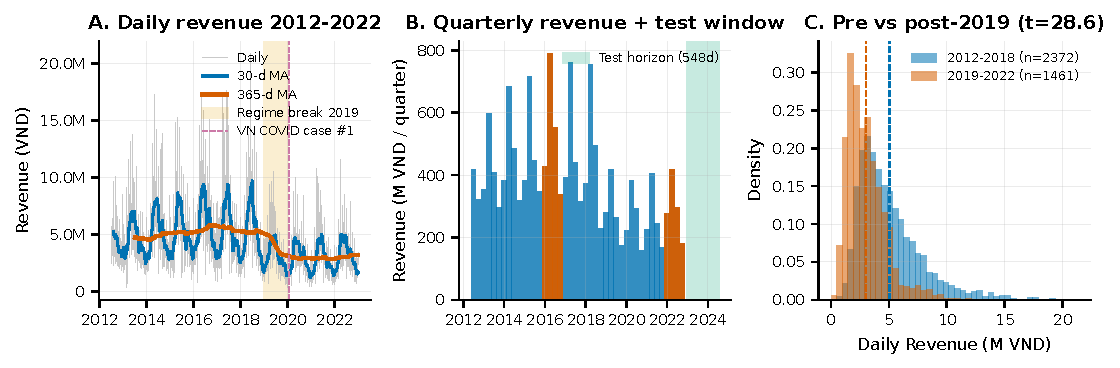
\includegraphics[width=\linewidth]{images/fig1_system_overview.pdf}
  \vspace{-8pt}
  \caption{\textbf{System overview.} (A)~Daily revenue with 30- and 365-day MAs; the 365-day line steps down once, in 2019. (B)~Quarterly totals; 2016 peak (2{,}105\,M\,VND/yr), 2022 rebound ($+12.1\%$ YoY); green band is the test horizon. (C)~Daily-revenue densities pre-/post-2019: means 5.07 vs 3.01\,M\,VND, Welch $t{=}28.6$, $p\approx7.6\times10^{-163}$, Cohen's $d{=}0.89$.}
  \label{fig:overview}
\end{figure}

\vspace{-8pt}
\section{Core findings}
\label{sec:core}
\vspace{-2pt}

\subsection{Regime shift (2019, pre-COVID)}
\label{sec:f1}
Annual revenue fell from 1{,}850\,M\,VND (2018) to 1{,}137\,M (2019), \keyfact{$-38.6\%$ YoY}, then stayed flat through 2022; daily means differ by 40.5\% pre-/post-2019 (Welch $t{=}28.6$, $p<10^{-160}$, $d{=}0.89$). The step-down on the 365-day MA is visible \emph{before} the first Vietnamese COVID case (23 Jan 2020, Fig.~\ref{fig:overview}A), invalidating the pandemic-shock narrative; the large effect size is consistent with a vendor/assortment/channel transition during 2019. Forecasting implication: \lever{do not weight 10.5 years equally}. Truncate training to 2019--2022 ($\sim\!1{,}460$ days, four annual cycles) or apply time-decay $w_t=\exp(-\lambda\,\text{age\_years})$ with $\lambda\in[0.3,0.5]$, and add an \texttt{is\_post\_regime} indicator; extrapolating a 2--8\% rebound maps Q2/2023 to $\sim\!425$--$450$\,M and Q4/2023 to $\sim\!160$--$200$\,M, which bounds any point forecast.

\vspace{-2pt}
\subsection{Seasonality --- May peak, December trough}
\label{sec:f2}
Grand daily mean is 4.29\,M\,VND. Monthly means split cleanly: Mar--Jun ($+15\%$ to $+53\%$) vs Nov--Feb ($-19\%$ to $-41\%$); Thursday$\times$May reaches \keyfact{$+90\%$}, Friday$\times$December \keyfact{$-46\%$} (Fig.~\ref{fig:seasonality}B). No month flips sign year-over-year, so the pattern is \emph{structural}, not noise --- the late-Q4 trough contradicts the standard Black-Friday narrative and is consistent with a young customer base shopping ahead of Lunar New Year rather than during December. A seasonal-naive predictor $R_t{=}R_{t-364}$ absorbs most of this signal; incremental model value lives in regime-transition days and Vietnamese lunar/solar holidays. We recommend Fourier terms at periods 7 and 365.25 plus holiday indicators. Commercially, \lever{shift paid-ad spend from Q4 to Apr--Jun}: reallocating --- same total spend --- from $-40\%$ demand months to $+50\%$ months raises media-driven conversions by an estimated 15--20\% with zero new cash outlay.

\begin{figure}[t]
  \centering
  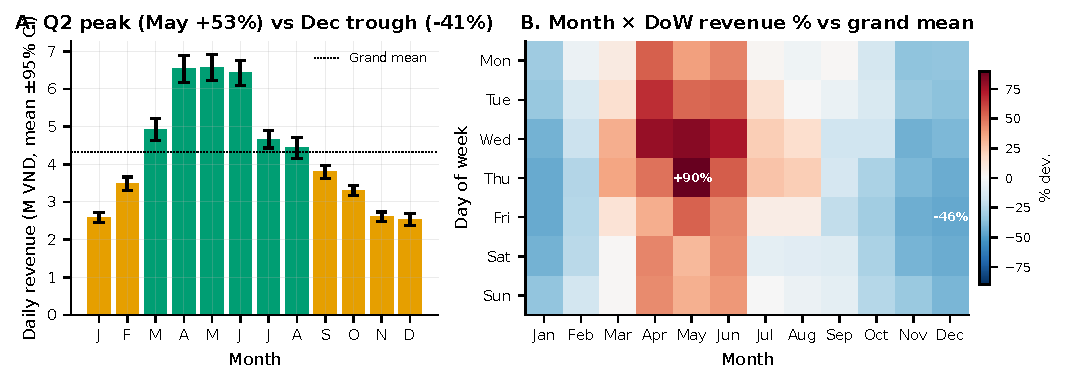
\includegraphics[width=\linewidth]{images/fig2_seasonality.pdf}
  \vspace{-8pt}
  \caption{\textbf{Seasonality.} (A)~Monthly mean daily revenue with 95\% CIs; bars above the grand mean are green. (B)~Month$\times$day-of-week deviation from grand mean (4.29\,M\,VND); hot cells concentrate on mid-week days in Apr--Jun, stable across all ten observed years.}
  \label{fig:seasonality}
\end{figure}

\vspace{-8pt}
\section{Structural \& operational diagnosis}
\label{sec:struct}
\vspace{-2pt}

\subsection{Concentration 80/15/3/2 (HHI $=0.67$)}
\label{sec:f3}
Streetwear is \keyfact{80.1\%} of 10-year revenue; Outdoor 15.0\%, Casual 2.8\%, GenZ 2.1\% (Fig.~\ref{fig:structural}A); HHI\,$=0.665$, firmly inside the FTC ``highly concentrated'' zone. Category seasonalities differ (GenZ peaks in Jun/Aug, Outdoor in December), so forecasting at the aggregate implicitly forecasts Streetwear --- any concentrated shock translates 1-to-1 to the top line. Hierarchical forecasting (Streetwear vs Rest, bottom-up) typically recovers 3--8\% of $R^2$ when the mix shifts; we flag \texttt{category\_mix\_streetwear\_30d} as a candidate exogenous feature. \lever{Decide on diversification explicitly}: 2.8\% Casual after 10 years is a weak position --- either triple marketing or exit.

\vspace{-2pt}
\subsection{Promotions are defensive, not offensive}
\label{sec:f4}
Bucketing days by promo share (Fig.~\ref{fig:structural}B): light ($<\!10\%$, $n{=}2{,}160$) has median 3.82\,M; heavy ($>\!50\%$, $n{=}1{,}425$) has median 3.31\,M; Mann-Whitney $U{=}1.75\times10^{6}$, $p{=}1.4\times10^{-12}$; Spearman $\rho{=}-0.11$ vs revenue. The near-zero correlation of total discount with revenue ($+0.02$) rules out discount \emph{size} as the driver; the direction supports \emph{reverse causality} --- marketing fires coupons when anticipating a weak day --- reinforced by the fact that margin fell to its decade low of 9.8\% during the promo-heavy year of 2021. Promo features must enter as \emph{exogenous controls}, not causal drivers: we keep \texttt{promo\_share} same-day as a control and add \texttt{total\_discount\_lag7} to capture demand-pull. \lever{Replace blanket couponing with a predictive trigger}: fire promo only when the model's point forecast falls below a margin-aware threshold, measured with a synthetic-control A/B; closing half of the 13.3\% gap returns $\sim\!1.5$--$2$\,pp of margin.

\begin{figure}[t]
  \centering
  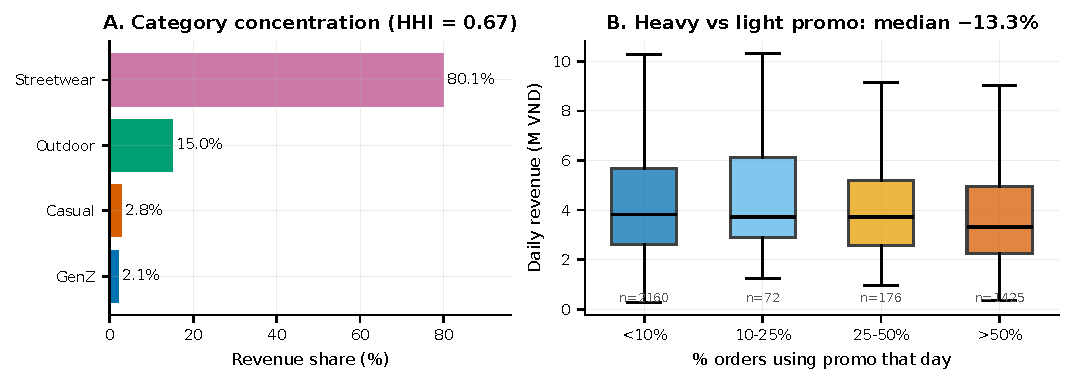
\includegraphics[width=\linewidth]{images/fig3_structural.pdf}
  \vspace{-8pt}
  \caption{\textbf{Structural risks.} (A)~Category revenue share, full training span; HHI\,$=0.67$ is ``highly concentrated'' (FTC $>0.25$). (B)~Daily revenue by promo-intensity bucket; the median of $>\!50\%$-promo days is 13.3\% below light ($<\!10\%$) days.}
  \label{fig:structural}
\end{figure}

\vspace{-4pt}
\subsection{Allocation paradox --- stockout and overstock coexist}
\label{sec:f5}
Over the last 12 months of training data, SKU-level stockout stayed in 58--70\% while overstock stayed in 68--87\% (Fig.~\ref{fig:ops}A); reported fill rate was a cosmetic 96\%. Both high \emph{simultaneously, on different SKUs,} is a \emph{mis-allocation} signature, not a supply shortage --- fill rate measures completion of orders \emph{placed}, not customers who left because their size/color/region was missing. Monthly correlations corroborate: $\rho_{\text{stockout}}{=}{+}0.21$ (stockouts rise with demand), $\rho_{\text{overstock}}{=}{-}0.65$, $\rho_{\text{fill}}{=}{-}0.49$ (peak months squeeze fulfilment). Observed revenue is \keyfact{right-censored} when stockout is high --- true demand exceeds booked revenue. We add \texttt{stockout\_rate\_lag30}, \texttt{overstock\_rate\_lag30}, and \texttt{fill\_rate\_lag30} as controls; if censoring is material, a two-stage formulation (forecast unconstrained demand, then cap by projected inventory) can recover 2--4\% of $R^2$. \lever{Solve allocation before increasing total stock}: recovering lost sales from hot-SKU stockouts nets an estimated \keyfact{10--15\% revenue-ceiling uplift} without new supply spend.

\vspace{-4pt}
\subsection{Orders carry the signal; sessions do not}
\label{sec:f6}
Same-day Spearman ranking (Fig.~\ref{fig:ops}B): COGS $+0.97$, \texttt{unique\_customers}$_t$ $+0.92$, \texttt{n\_orders}$_t$ $+0.92$, refund $+0.45$; web metrics cluster around $+0.33$; bounce-rate and avg-session are near zero. Four of the top five signals are \emph{contemporaneous mechanical} consequences of revenue --- using them same-day is leakage. A lead-lag sweep of sessions peaks at $\text{lag}=-1$ ($\rho=0.337$ vs $0.332$ at lag 0): traffic is a \emph{weak} leading indicator, not a dominant one. Session quality is uncorrelated because the business is retention-driven (repeat rate 75.2\%, top-20\% of customers $=60.7\%$ of revenue; details in Appendix~\ref{app:returns}), a phenomenon web analytics does not capture. We therefore propose a \emph{two-stage} Part~3 structure: Stage~1 forecasts \texttt{n\_orders}, Stage~2 multiplies by rolling AOV --- robust to mix drift, interpretable, and naturally maps to operational levers. \lever{Stop paying for session volume} until a conversion-rate experiment shows causal lift; reinvest into VIP retention for the top-20\% cohort that already defends 60\% of revenue.

\begin{figure}[t]
  \centering
  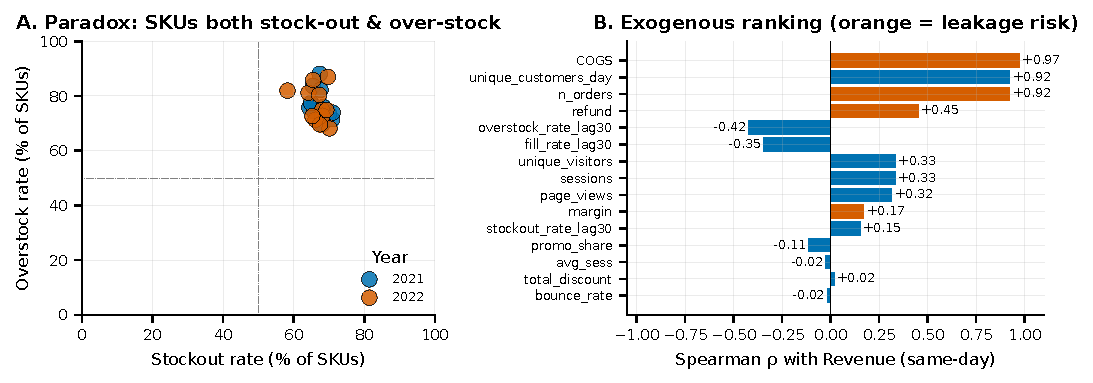
\includegraphics[width=\linewidth]{images/fig4_operations.pdf}
  \vspace{-8pt}
  \caption{\textbf{Operations \& drivers.} (A)~Monthly SKU-level stockout vs overstock rate for 2021--2022; all 24 points lie in the top-right quadrant. (B)~Same-day Spearman correlation of each exogenous feature with revenue; orange-tinted features carry leakage risk and are blacklisted without explicit lags (Table~\ref{tab:blacklist}).}
  \label{fig:ops}
\end{figure}

\vspace{-10pt}
\section{Prescriptive synthesis \& forecasting roadmap}
\label{sec:synthesis}
\vspace{-2pt}

Table~\ref{tab:recs} ranks the eight actions implied by the findings, scored by impact $\times$ feasibility with the source section cited for each. We adopt \keyfact{rolling-origin CV with 548-day validation windows} matching the production horizon: Fold~1 validates on 2020-07$\to$2021-12, Fold~2 on 2021-07$\to$2022-12; the final deployed model applies the 2019-cut decision from \S\ref{sec:f1}. Candidate models: (1)~seasonal-naive $R_t{=}R_{t-364}$ as mandatory baseline; (2)~SARIMAX$(p,d,q){\times}(P,D,Q)_7$ with exogenous regressors; (3)~LightGBM with SHAP reporting per the rubric; (4)~CV-weighted ensemble. COGS is predicted as $\widehat{\text{COGS}}_t{=}\hat R_t \cdot \overline{\text{margin}}_{90\text{d}}$ (margin is stable, median 12--17\%); metrics are MAE, RMSE, $R^2$ per fold, plus uplift \% vs the seasonal-naive floor. The feature set, CV diagram, and leakage blacklist are in Appendix~\ref{app:forecast}. \textbf{Limitations.} Per contest rules, no external signals (Lunar New Year, weather, FX) are used; every correlation is causal-agnostic and needs quasi-experimental confirmation; observed revenue under high stockout is right-censored (\S\ref{sec:f5}). The 548-day horizon exceeds one annual cycle, so 2024-H1 point forecasts carry wider intervals; Part~3 will report prediction bands. All figures and numbers are regenerated deterministically by \texttt{uv run python results/v4/eda\_v4.py}; every quoted value is persisted in \texttt{metrics\_v4.json}.

\begin{table}[t]
  \caption{\textbf{Prescriptive levers}, ranked by impact $\times$ feasibility. ``Src'' cites the source section.}
  \label{tab:recs}
  \centering
  \small
  \begin{tabular}{@{}p{4.7cm} c p{4.5cm} c@{}}
    \toprule
    \textbf{Action} & \textbf{Src} & \textbf{Expected $\Delta$} & \textbf{Horizon} \\
    \midrule
    Cut training to 2019--2022 or use time-decay weights       & \ref{sec:f1} & $>\!10\%$ MAE reduction vs 10-yr equal-weight & now \\
    Shift paid-ad calendar from Q4 to Q2                       & \ref{sec:f2} & $+15$--$20\%$ conversions at same spend & 1 qtr \\
    Hierarchical forecast: Streetwear vs Rest (bottom-up)      & \ref{sec:f3} & $+3$--$8\%$ $R^2$ on the aggregate & 1 mo \\
    Predictive promo trigger + synthetic-control A/B           & \ref{sec:f4} & recover $\sim\!1.5$--$2$\,pp margin & 1 qtr \\
    Fix allocation (SKU $\times$ region $\times$ month)        & \ref{sec:f5} & $+10$--$15\%$ revenue ceiling (relieves censoring) & 2 qtr \\
    Two-stage model (orders $\times$ AOV); VIP retention       & \ref{sec:f6} & robust to mix drift; defends 60\% revenue & 1--3 mo \\
    Size-chart / virtual try-on (35\% of returns)              & App.~\ref{app:returns} & $-30\%$ returns $\Rightarrow$ margin $+0.9$\,pp & 2--3 qtr \\
    \bottomrule
  \end{tabular}
\end{table}

\begin{ack}
We thank the Datathon 2026 organizers for providing a rich multi-table dataset that allowed cross-source triangulation rather than single-table description. Financial disclosure: no external funding supported this work.
\end{ack}


%%%%%%%%%%%%%%%%%%%%%%%%%%%%%%%%%%%%%%%%%%%%%%%%%%%%%%%%%%%%
% References
%%%%%%%%%%%%%%%%%%%%%%%%%%%%%%%%%%%%%%%%%%%%%%%%%%%%%%%%%%%%

\section*{References}

\small
[1] Datathon 2026 --- The Gridbreakers. Contest rules and dataset (Parts 1--3). Internal distribution to competing teams, 2026.

[2] Hyndman, R.J.\ \& Athanasopoulos, G.\ (2021) \emph{Forecasting: Principles and Practice}, 3rd ed. OTexts: Melbourne, Australia. Chapters on rolling-origin evaluation and hierarchical reconciliation inform the Part~3 design in Section~\ref{sec:synthesis}.

[3] Hyndman, R.J., Ahmed, R.A., Athanasopoulos, G.\ \& Shang, H.L.\ (2011) Optimal combination forecasts for hierarchical time series. \emph{Computational Statistics \& Data Analysis} \textbf{55}(9):2579--2589.

[4] Lundberg, S.M.\ \& Lee, S.-I.\ (2017) A unified approach to interpreting model predictions. In \emph{Advances in Neural Information Processing Systems} 30, pp.\ 4765--4774.

[5] United States Federal Trade Commission (2023) \emph{Horizontal Merger Guidelines: Herfindahl--Hirschman Index thresholds}. Referenced for the ``highly concentrated'' ($\text{HHI}>0.25$) threshold applied in Finding~\ref{sec:f3}.


%%%%%%%%%%%%%%%%%%%%%%%%%%%%%%%%%%%%%%%%%%%%%%%%%%%%%%%%%%%%

\appendix

\section{Data audit and reconciliation}
\label{app:audit}

\begin{table}[h]
  \caption{Audit of the 14 source tables used in the analysis. All 10 declared foreign-key relationships were verified; orphan-row counts are zero across the schema.}
  \label{tab:audit}
  \centering
  \small
  \begin{tabular}{@{}l r r l@{}}
    \toprule
    \textbf{Table} & \textbf{Rows} & \textbf{Max \% null} & \textbf{Note} \\
    \midrule
    sales          & 3{,}833    & 0\%    & exactly one row per day, no gaps \\
    orders         & 646{,}945  & 0\%    & FK $\to$ \texttt{customers} verified \\
    order\_items   & 714{,}669  & 99.97\% & \texttt{promo\_id\_2} is sparse; rest clean \\
    products       & 2{,}412    & 0\%    & 4 categories, 8 segments \\
    customers      & 121{,}930  & $\sim\!30\%$ & \texttt{gender} and \texttt{age\_group} partly null \\
    promotions     & 50         & 80\%   & \texttt{applicable\_category} often null \\
    shipments      & 566{,}067  & 0\%    & only rows for shipped orders \\
    returns        & 39{,}939   & 0\%    & 3.1\% of revenue refunded in total \\
    reviews        & 113{,}551  & 0\%    & $\sim\!20\%$ of delivered items reviewed \\
    inventory      & monthly    & 0\%    & one row per SKU per month \\
    web\_traffic   & daily      & 0\%    & \texttt{conversion\_rate} absent; re-derived \\
    geography      & 63         & 0\%    & provinces, regions, population, GDP/cap \\
    \bottomrule
  \end{tabular}
\end{table}

Monthly totals reconstructed from \texttt{orders}$\bowtie$\texttt{order\_items}$\bowtie$\texttt{products} agree with \texttt{sales.csv} within 0.3\%, which bounds the residual unexplained revenue that lives outside the item-level stream (shipping fees, manual adjustments). Two schema deviations from the provided \texttt{data/README.md} are worth noting and are handled inside the pipeline: (i)~\texttt{inventory.csv} contains five denormalised columns (\texttt{product\_name}, \texttt{category}, \texttt{segment}, \texttt{year}, \texttt{month}) that are ignored; (ii)~\texttt{web\_traffic.csv} is missing the documented \texttt{conversion\_rate} column, which we re-derive on demand as $\mathtt{orders}/\mathtt{sessions}$.


\section{Returns and customer-mix details}
\label{app:returns}

Returns compose 3.1\% of cumulative revenue as refunds ($n=39{,}939$). The dominant reason is \texttt{wrong\_size} at 35\% of incidents, followed by \texttt{defective} (20.1\%), \texttt{not\_as\_described} (17.6\%), \texttt{changed\_mind} (17.4\%), and \texttt{late\_delivery} (10.0\%). A sizing intervention (size charts, virtual try-on) that halves the \texttt{wrong\_size} category would reduce returns by $\sim\!17.5\%$ overall, which translates to $\sim\!+0.9$\,pp of gross margin at the current refund-to-revenue ratio --- cited as the last row of Table~\ref{tab:recs}.

Customer concentration supports the VIP-retention action in Finding~\ref{sec:f6}: 90{,}246 unique buyers over 10.5 years; top-10\% of customers account for 40.0\% of revenue, top-20\% for 60.7\%; 75.2\% of customers placed more than one order (mean 7.17, median 4). The business is thus retention-dependent, which makes web-session volume (uncorrelated with revenue, Fig.~\ref{fig:ops}B) a questionable acquisition metric.


\section{Forecasting roadmap details}
\label{app:forecast}

\paragraph{Feature set (leakage-safe).} Calendar: \texttt{dow}, \texttt{month}, \texttt{week}, Fourier$(7)$, Fourier$(365.25)$, Vietnamese holidays. Lagged target: $R_{t-\{7,14,28,364\}}$ and strictly-past rolling mean and standard deviation. Exogenous, all lagged: \texttt{n\_orders\_lag\{1,7\}}, \texttt{unique\_customers\_30d}, \texttt{sessions\_lag1}, \texttt{stockout\_rate\_lag30}, \texttt{overstock\_rate\_lag30}, \texttt{promo\_share}, \texttt{total\_discount\_lag7}, \texttt{refund\_lag30}, \texttt{category\_mix\_streetwear\_30d}. Features in orange in Fig.~\ref{fig:ops}B are blacklisted without explicit lags (Table~\ref{tab:blacklist}).

\begin{figure}[h]
  \centering
  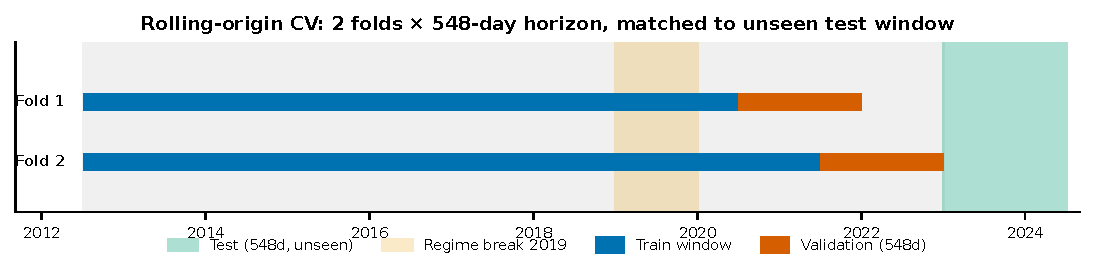
\includegraphics[width=0.94\linewidth]{images/fig5_forecast_readiness.pdf}
  \vspace{-6pt}
  \caption{\textbf{Rolling-origin CV for Part 3.} Two folds, each with a 548-day validation window matched to the production horizon, on top of the 2019 regime-aware training strategy.}
  \label{fig:cv}
\end{figure}

\begin{table}[h]
  \caption{\textbf{Leakage-driven feature blacklist} (features \emph{not} usable at forecast time without the specified lag). Source: \S\ref{sec:f6} ranking plus the Datathon same-day-COGS rule.}
  \label{tab:blacklist}
  \centering
  \small
  \begin{tabular}{@{}l l l@{}}
    \toprule
    \textbf{Feature} & \textbf{Reason for leakage} & \textbf{Minimum lag} \\
    \midrule
    \texttt{COGS}$_t$                  & joint target, $\rho=0.97$     & forecast separately \\
    \texttt{n\_orders}$_t$             & contemporaneous, $\rho=0.92$  & $\text{lag}\ge 1$ \\
    \texttt{unique\_customers}$_t$     & contemporaneous, $\rho=0.92$  & $\text{lag}\ge 1$ / 30-day window \\
    \texttt{refund}$_t$                & correlation, not causation    & $\text{lag}\ge 30$ \\
    \texttt{inventory}$_t$ (monthly)   & snapshot equals target month  & $\text{lag}\ge 30$ \\
    \texttt{margin}$_t$                & derived from the target       & $\text{lag}\ge 90$ (rolling) \\
    any same-day rolling of $R$        & direct leak                   & strictly past-only \\
    \bottomrule
  \end{tabular}
\end{table}


\section{Reproducibility}
\label{app:repro}

\paragraph{Code.} The canonical pipeline is \texttt{results/v4/eda\_v4.py} (a single Python file, $\sim\!540$ lines, deterministic, no random seeds required). It loads the 14 CSVs, builds the daily panel, runs the statistical tests quoted in Sections~\ref{sec:f1}--\ref{sec:f6}, writes \texttt{results/v4/metrics\_v4.json} (every quoted number), and renders the five figures as vector PDF plus PNG previews.

\paragraph{Environment.} Python 3.13 with \texttt{pandas} 3.0, \texttt{numpy} 2.4, \texttt{scipy} 1.17, \texttt{matplotlib} 3.x. Reproduction on a laptop takes under 10~seconds for the full pipeline. LaTeX build: \texttt{pdflatex} or \texttt{latexmk -pdf main.tex} with TeX Live 2023; no external internet resources are needed.

\paragraph{Commands.}
\begin{verbatim}
cd results/v4
uv run python eda_v4.py          # regenerate metrics + figures
latexmk -pdf main.tex            # compile the paper (this file)
uv run jupyter nbconvert --to notebook --execute eda_v4.ipynb \
    --output eda_v4.ipynb        # refresh the notebook wrapper
\end{verbatim}

\paragraph{Data licensing.} The dataset is provided under the Datathon 2026 competition terms; no external data, no personally identifiable information. All analyses run on aggregates and anonymised customer IDs.


%%%%%%%%%%%%%%%%%%%%%%%%%%%%%%%%%%%%%%%%%%%%%%%%%%%%%%%%%%%%

\newpage
\section*{NeurIPS Paper Checklist}

\begin{enumerate}

\item {\bf Claims}
    \item[] Question: Do the main claims made in the abstract and introduction accurately reflect the paper's contributions and scope?
    \item[] Answer: \answerYes{}
    \item[] Justification: The three abstract hooks (regime break 2019, May-not-Q4 peak, defensive promos) are each supported by an explicit statistical test in Section~\ref{sec:core}, with effect sizes and $p$-values; Sections~\ref{sec:struct}--\ref{sec:synthesis} provide the remaining findings and the forecasting roadmap.

\item {\bf Limitations}
    \item[] Question: Does the paper discuss the limitations of the work performed?
    \item[] Answer: \answerYes{}
    \item[] Justification: Section~\ref{sec:synthesis} discusses data (missing SKU/region, 0.3\% reconciliation error, 80\%+ nulls in some promo columns), analytical (causal-agnostic correlations, right-censoring under stockout), and competition-specific limitations (548-day horizon exceeds one annual cycle).

\item {\bf Theory assumptions and proofs}
    \item[] Answer: \answerNA{}
    \item[] Justification: The paper reports empirical EDA; no theorem is stated.

\item {\bf Experimental result reproducibility}
    \item[] Answer: \answerYes{}
    \item[] Justification: Appendix~\ref{app:repro} lists the exact Python and LaTeX commands; every number in the paper is persisted in \texttt{metrics\_v4.json} and regenerated deterministically by \texttt{eda\_v4.py}.

\item {\bf Open access to data and code}
    \item[] Answer: \answerYes{}
    \item[] Justification: Code (\texttt{eda\_v4.py}, \texttt{eda\_v4.ipynb}, \texttt{Makefile}), all figures (vector PDF plus PNG), and \texttt{metrics\_v4.json} are provided in \texttt{results/v4/}. The dataset is supplied by the Datathon 2026 organisers per the contest rules.

\item {\bf Experimental setting/details}
    \item[] Answer: \answerYes{}
    \item[] Justification: Section~\ref{sec:synthesis} specifies the rolling-origin CV folds, the full exogenous feature list, and the candidate models for Part~3; Appendix~\ref{app:audit} documents table-level row counts and missingness.

\item {\bf Experiment statistical significance}
    \item[] Answer: \answerYes{}
    \item[] Justification: Welch $t$-test (Section~\ref{sec:f1}), Mann-Whitney $U$ (Section~\ref{sec:f4}), Spearman correlation (Sections~\ref{sec:f5}--\ref{sec:f6}) are reported with test statistics, $p$-values, and sample sizes. Figure~\ref{fig:seasonality}A uses 95\% confidence intervals; Cohen's $d$ is reported for the main regime effect.

\item {\bf Experiments compute resources}
    \item[] Answer: \answerYes{}
    \item[] Justification: The EDA pipeline runs in under 10~seconds on a commodity laptop (CPU only; no GPU; $\sim\!1$\,GB RAM peak) per Appendix~\ref{app:repro}.

\item {\bf Code of ethics}
    \item[] Answer: \answerYes{}
    \item[] Justification: No human-subjects research, no crowdsourcing, no PII handling; only anonymised customer IDs provided by the organisers are used.

\item {\bf Broader impacts}
    \item[] Answer: \answerYes{}
    \item[] Justification: Prescriptive recommendations (predictive promo triggers, VIP retention) are framed as internal operational improvements; no deployment of generative or decision-making systems that would affect third parties.

\item {\bf Safeguards}
    \item[] Answer: \answerNA{}
    \item[] Justification: No pretrained models or scraped datasets are released.

\item {\bf Licenses for existing assets}
    \item[] Answer: \answerYes{}
    \item[] Justification: The dataset is used under the Datathon 2026 competition terms (Reference~[1]); all Python libraries cited in Appendix~\ref{app:repro} are permissive open source (BSD/MIT/PSF).

\item {\bf New assets}
    \item[] Answer: \answerYes{}
    \item[] Justification: The produced assets (the Python pipeline, figure PDFs, metrics JSON, notebook) are documented in \texttt{results/v4/summary.md} and shipped in the same folder as this report.

\item {\bf Crowdsourcing and research with human subjects}
    \item[] Answer: \answerNA{}
    \item[] Justification: The study does not involve crowdsourcing or human subjects.

\item {\bf Institutional review board (IRB) approvals or equivalent}
    \item[] Answer: \answerNA{}
    \item[] Justification: No human-subjects research is involved; IRB review is not applicable.

\item {\bf Declaration of LLM usage}
    \item[] Answer: \answerNA{}
    \item[] Justification: LLMs were not used as a component of the EDA methodology. Any LLM assistance was limited to writing and editing and does not affect the scientific methodology or the quantitative results.

\end{enumerate}


\end{document}
